\chapter{Reconoces las propiedades de la circunferencia}

\section{Rectas y segmentos}

\subsection{Definición}

La circunferencia de un un círculo es el conjunto de los puntos del plano que
equidistan el centro.

\begin{center}
 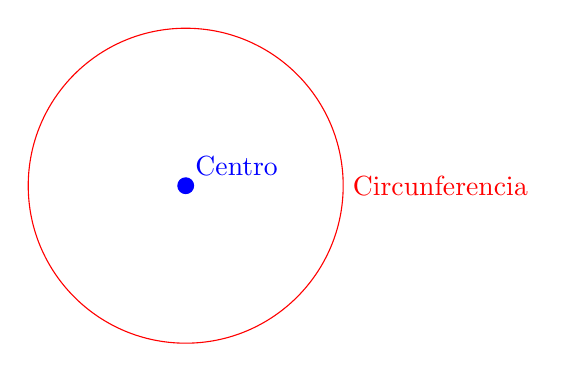
\begin{tikzpicture}
   \draw[color=blue] (0,0) node[above right]{Centro} circle(.1)[fill=blue];
   \draw[color=red] (0,0)  circle(2) (2,0) node[right] {Circunferencia};
 \end{tikzpicture}
\end{center}

Un radio es un segmento que une el centro con otro punto de la circunferencia.

\begin{center}
 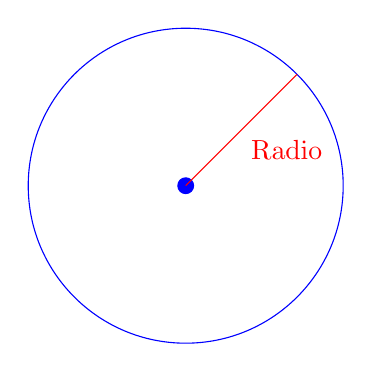
\begin{tikzpicture}
   \draw[color=blue] (0,0) circle(.1)[fill=blue];
   \draw (0,0)  circle(2)[color=blue];
   \draw[color=red]
   (0,0) -- (0.70710678118654,0.70710678118654)node[below right]{Radio} --
   (1.414213562373095,1.414213562373095);
 \end{tikzpicture}
\end{center}

Un diámetro es un segmento que une dos puntos en circunferencia y que pasa
por el centro. Si $R$ es la longitud de un radio, los diámetros median
$2R$.

\begin{center}
 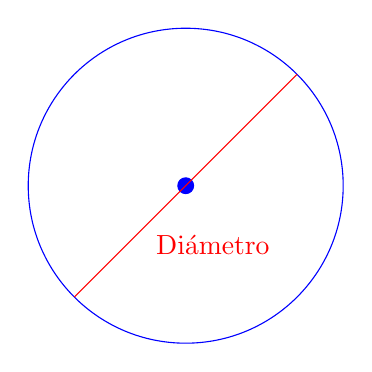
\begin{tikzpicture}
   \draw[color=blue] (0,0) circle(.1)[fill=blue];
   \draw[color=blue] (0,0)  circle(2) (2,0);
   \draw[color=red]
   (-1.414213562373095,-1.414213562373095) --
   (0,0) -- (-0.5,-0.5)node[below right]{Diámetro} --
   (1.414213562373095,1.414213562373095);
 \end{tikzpicture}
\end{center}

De manera más general, un segmento que une dos puntos en circunferencia se
llama un cuerda.

\begin{center}
 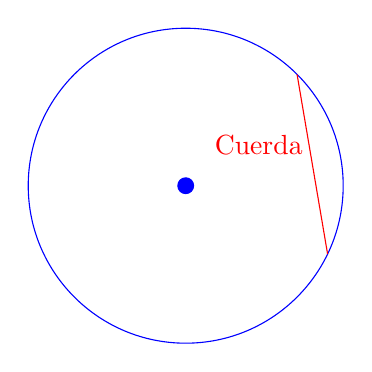
\begin{tikzpicture}
   \draw[color=blue] (0,0) circle(.1)[fill=blue];
   \draw[color=blue] (0,0)  circle(2) (2,0);
   \draw[color=red]
   (1.801937735804838,-0.86776747823511) --
   (1.608075649088966,0.27322304206898)node[above left]{Cuerda} --
   (1.414213562373095,1.414213562373095);
 \end{tikzpicture}
\end{center}

Una cuerda divide la circunferencia en dos partes llamadas arcos.

\begin{center}
 \begin{tikzpicture}
   \draw[color=blue] (0,0) circle(.1)[fill=blue];
   \draw[color=blue]
   (1.801937735804838,-0.86776747823511) --
   (1.414213562373095,1.414213562373095);

   \draw[color=red] (1.414213562373095,1.414213562373095)
   arc(45:0:2) node[above right]{Arco}
   arc(0:-25.71428571428571:2);

   \draw[color=orange] (1.414213562373095,1.414213562373095)
   arc(45:200:2) node[below left]{Arco}
   arc(200:334.2857142857143:2);

 \end{tikzpicture}
\end{center}

Para un diámetro, los dos arcos son llamados semicircunferencia.

\begin{center}
 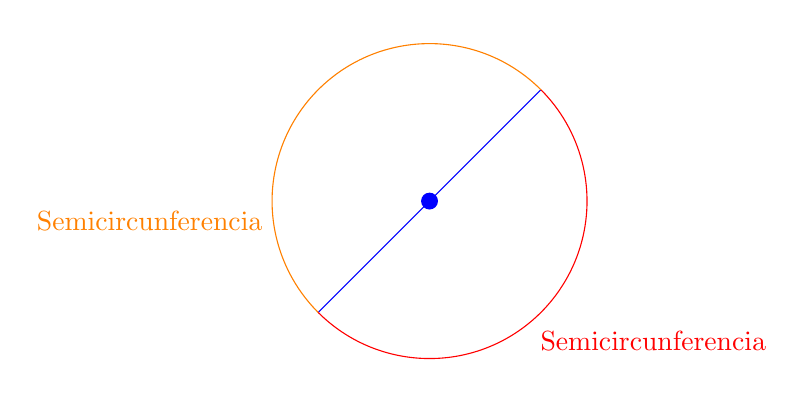
\begin{tikzpicture}
   \draw[color=blue] (0,0) circle(.1)[fill=blue];
   \draw[color=blue]
   (1.414213562373095,1.414213562373095) --
   (-1.414213562373095,-1.414213562373095);

   \draw[color=red] (1.414213562373095,1.414213562373095)
   arc(45:-50:2) node[below right]{Semicircunferencia}
   arc(-50:-135:2);

   \draw[color=orange] (1.414213562373095,1.414213562373095)
   arc(45:180:2) node[below left]{Semicircunferencia}
   arc(180:225:2);

 \end{tikzpicture}
\end{center}

Una recta pasando por dos puntos de una circunferencia es dicha secante.
Una recta que no corta la circunferencia es dicha exterior. Si corta
la circunferencia en exactamente un punto es dicha tangente, y es ortogonal
al radio corespondiente.

\begin{center}
 \begin{tikzpicture}
   \draw[color=blue] (0,0) circle(.1)[fill=blue];
   \draw[color=blue] (0,0) circle(2) (2,0);
   \draw[color=red] (-2,-2) -- (-1,3) node[above right] {Secante};
   \draw[color=red] (3,-3) -- (5,3) node[above right] {Exterior};

   \begin{scope}[rotate around={-10:(0,0)}]
   \draw[color=blue] (2,0) circle(.1)[fill=blue];
   \draw[color=red] (2,-4) -- (2,4) node[above right] {Tangente};
   \draw[color=orange](1.8,0) -- (1.8,.2) -- (2,.2);
   \draw[color=orange](0,0) -- (2,0);
   \end{scope}

 \end{tikzpicture}
\end{center}

\subsection{Ejercicio 1}

En este ejercicio, consiramos un segmento $[AB]$ y utilizamos
regla y compás.

\begin{center}
 \begin{tikzpicture}
   \draw[color=blue] (0,0) node[above]{$A$} -- (4,0) node[above]{$B$};
 \end{tikzpicture}
\end{center}

\begin{enumerate}
\item Determine el centro $O$ del círculo de diámetro $[AB]$, la
circunferencia del círculo y un radio $[OC]$ ortogonal a $[AB]$.

\item Indique la semicircunferencia asociada al diámetro $[AB]$ que no contene
$C$. Trace la cuerda $BC$ y el menor arco que delimita.
Compare la longitud de estes circunferencia, semicircunferencia y arco.

\item Trace la tangente en $C$. ¿Que decir de su posición relativa a $(AB)$?

\item Trace $D$ el simétrico de $A$ respecto a la tangente en $C$.
  De manera gráfica, encuentre la posición relativa a la circunferencia, de
  ¿la recta $(OD)$?, ¿la recta pasando por $D$ y paralela a $(OC)$?
  ¿la recta pasando por $D$ y paralela a $(AC)$?
\end{enumerate}

\section{Ángulos}

\subsection{Definición}

Wikipedia da las definiciones siguientes de
para un ángulo,respecto de una circunferencia:

\begin{enumerate}
\item Ángulo central, si tiene su vértice en el centro de esta. Sus lados
  contienen a dos radios.
\item Ángulo inscrito, si su vértice es un punto de la circunferencia y sus
  lados contienen dos cuerdas.
\item Ángulo semi-inscrito, si su vértice es un punto de la circunferencia y
  sus lados contienen una cuerda y una recta tangente a la circunferencia. El
  vértice es el punto de tangencia.
\item Ángulo interior, si su vértice está en el interior de la circunferencia.
\item Ángulo exterior, si tiene su vértice en el exterior de la circunferencia
\end{enumerate}

\subsection{Ejercicio 2}

Consideramos un círculo de centro $O$
y un recta secante, pasando por dos puntos $A,B$ del
círculo. Sea $C$ el medio del segmento $[OA]$ y el simétrico de $D$
respecto a la tangente en $B$.

\begin{itemize}
\item Indique si los ángulos $\widehat{ACB}$ y $\widehat{ADB}$ son
  interior o exterior.
\item Dibuje el ángulo central cuyo los lados pasan por $A,B$.
\item Dibuje el ángulo inscrito cuyo los lados pasan por $A,B,C$ pero no pasan
  por el centro $O$. Sea $E$ su vértice.
\item Dijube un ángulo semi-inscrito  de vértice $E$ y cuyo los lados
  contienen la cuerda $[EA]$.
\end{itemize}

\subsection{Ejercicio 3}

Consideramos un círculo de centro $O$ y dos puntos $A,B$ de la circunferencia.
Sea $M$ un punto de la circunferencia diferente de $A,B$.

\begin{enumerate}
\item La recta $(MO)$ intersecta el círculo en un punto $D \neq M$.
  ¿Que decir de la relación entre los ángulos $\widehat{AOD}$ y $\widehat{AOM}$?
  ¿Y entre los ángulos $\widehat{OAM}$ y $\widehat{AMO}$?
  Deduzca $2 \widehat{AMD} = \widehat{AOD}$.
\item ¿Cuál es la relación entre $\widehat{BMD}$ y $\widehat{BOD}$?
\item Consideramos las semicircunferencias asociadas al diámetro $[MD]$.
  Exprese $\widehat{AMB}$ en función de
  $\widehat{AMD}$ y $\widehat{BMD}$ según que $A,B$ sean sobre la misma
  semicircunferencias o no.
\item De la misma manera, Exprese $\widehat{AOB}$ en función de
  $\widehat{AOD}$ y $\widehat{BOD}$.
\item Deduzca el teorema del ángulo central: $2 \widehat{AMB} = \widehat{AOB}$.
\item Deduzca el teorema del ángulo inscrito: dos ángulos inscritos que
  abarcan el mismo arco son iguales.
\item Sea $H$ el medio de $[AB]$ y $T$ la tangente en $A$.
  ¿Que decir de las rectas $(HO)$ y $(BA)$?  ¿Y de las rectas $(OA)$ y $T$?
\item Deduzca que uno de los ángulos semi-inscrito de lado $[AB]$ y vértice
  $A$ es de misma amplitud que $\widehat{HOB}$.
\item Deduzca que este ángulo semi-inscrito es igual al ángulo
  inscrito $\widehat{AMB}$.
\end{enumerate}

\section{Perímetro y área}

La longitud de una circuferencia es proporcional a la longitud $2r$ de
su diámetro:
s
$$
L = \pi \times 2r
$$

La constante de proporcionalidad es el ńumero irracional
%%
$$\pi \approx 3.14159265358979323846$$

Como hemos visto en el ejercicio 9 del capítulo IV, la área del círculo es
%%
$$
A = \pi \times r^2
$$

Por consecuencia, si consideramos un ángulo central de amplitud $\alpha$
($0° \leq \alpha \leq 360°$), la longitud del arco que abarca es
%%
$$
L_{\alpha} = \pi \times 2r \times \frac{\alpha}{360°}
$$
%%
y la área del sector circular que determina es
%%
$$
A_{\alpha} = \pi \times r^2 \times \frac{\alpha}{360°}
$$

\subsection{Ejercicio 4}

Calcule una aproximación de

\begin{enumerate}
\item La longitud del círculo central de un terreno de fútbal (radio: $9.15$m).
\item La área de un disco compacto (diámetro: $12$cm)
\item La longitud del arco corespondiente a un radio de $R=2$m y ángulo
$\alpha=35$°.
\item La área de un sector corespondiente a un radio de $R=3$m y ángulo
$\alpha=75$°.
\end{enumerate}

\subsection{Ejercicio 5}

Sea una pizza de espesor $A = 5$mm y de radio $Z = 13$cm.
Utilizamos la aproximación $\pi \approx \mathrm{PI} = 3.14$.
¿Que representa $\mathrm{PI} \times Z \times Z \times A$? Determine su valor.

\section{Soluciones de los ejercicios}

\subsection{Ejercicio 1}

\begin{enumerate}
  \item El centro de $O$ es el medio del segmento $[AB]$ entonces podemos
    construirlo con la técnica de la mediatriz (Ejercicio 5,
    capítulo 3). Despues podemos trazar con
    el compás la circunferencia de radio $OA$. La mediatriz intersecta
    esta circunferencia en dos puntos, elegimos un punto $C$.

    \begin{center}
 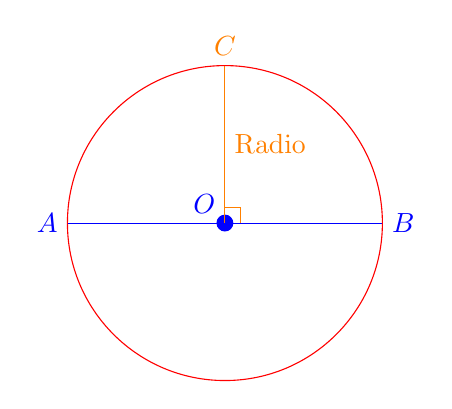
\begin{tikzpicture}
   \draw[color=blue] (-2,0) node[left]{$A$} -- 
   (0,0) node[above left]{$O$} -- (2,0) node[right]{$B$};
   \draw[color=blue] (0,0) circle(.1)[fill=blue];
   \draw[color=red] (0,0) circle(2);
   \draw[color=orange] (0,0) -- (0,1) node[right]{Radio} --
   (0,2) node[above]{$C$} (0,.2) -- (.2,.2) -- (.2,0);
 \end{tikzpicture}
\end{center}
    
    \item La longitud de la semicircunferencia es la mitad de la longitud de la
      circunferencia, y la longitud del arco es un cuarto de la longitud de la
      circunferencia.
    \begin{center}
 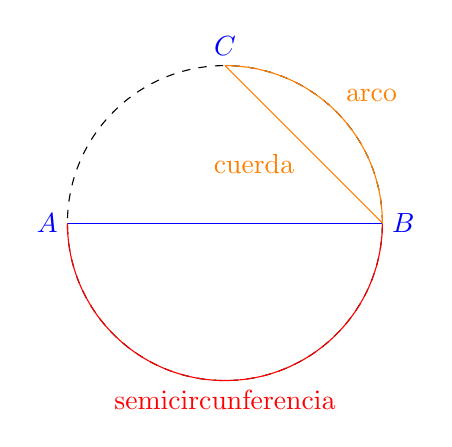
\begin{tikzpicture}
   \draw[dashed] (0,0) circle(2);
   \draw[color=blue] (-2,0) node[left]{$A$} -- (2,0) node[right]{$B$}
   (0,2) node[above]{$C$};
   \draw[color=red] (-2,0) arc(180:270:2) node[below]{semicircunferencia}
   arc(270:360:2);

   \draw[color=orange] (0,2) -- (1,1) node[below left]{cuerda}
   -- (2,0) arc(0:45:2) node[above right]{arco}  arc(45:90:2);
    \end{tikzpicture}
\end{center}

 \item Para trazar la tangente, utilizamos la técnica para construir
   una recta ortogonal a $(OC)$ y pasando por el punto $C$ (Ejercicio 5,
   capítulo 3). Por que $(AC)$ es ortogonal a $(OC)$ y
   $C \notin (AB)$ la tangente es paralela a $(AB)$.

    \begin{center}
    \begin{tikzpicture}
   \draw[color=blue] (-2,0) node[left]{$A$} -- 
   (0,0) node[above left]{$O$} -- (2,0) node[right]{$B$} (0,2) node[above]{$C$};
   \draw[color=blue] (0,0) circle(.1)[fill=blue];
   \draw[color=red] (0,0) circle(2);
   \draw[color=orange] (0,0) --
   (0,2) (0,.2) -- (.2,.2) -- (.2,0);
   \draw[color=green] (-4,2) --
   (2,2) node[above]{Tangente} -- (4,2);

    \end{tikzpicture}
\end{center}

\item Son respectivamente secante, tangente y exterior a la circuferencia.

    \begin{center}
    \begin{tikzpicture}
   \draw[color=blue] (-2,0) node[left]{$A$} -- 
   (0,0) node[above left]{$O$} -- (2,0) node[right]{$B$} (0,2) node[above]{$C$};
   \draw[color=blue] (0,0) circle(.1)[fill=blue];
   \draw[color=red] (0,0) circle(2);
   \draw[color=orange] (0,0) --
   (0,2) (0,.2) -- (.2,.2) -- (.2,0);
   \draw[dashed] (-4,2) -- (4,2);
   \draw[color=blue] (-2,4) node[right]{$D$} circle(.1)[fill=blue];

   \draw[color=green] (-3,6) -- (1,-2);
   \draw[color=green] (-2,6) -- (-2,-2);
   \draw[color=green] (0,6) -- (-6,0);
    \end{tikzpicture}
\end{center}

\end{enumerate}

\subsection{Ejercicio 2}

\begin{itemize}
\item $\widehat{ACB}$ es un ángulo interior (porque $C$ es el medio de del radio
  $[OA]$ y entonces en el interior del círculo) mientras que
  $\widehat{ADB}$ es un ángulo exterior (porque $C$ está en el semi-plano
  delimitado por $T$ que contene el ćirculo y entonces $D$ es en el otro
  semi-plano que no contene el ćirculo).
\item Es el ángulo $\widehat{AOB}$ ázul.
\item El el ángulo $\widehat{AEB}$ naranja (la otra posibilidad
  $C \in (EA)$ implica $O \in (EA)$)
\item La tangente en $E$ (amarilla) se compone de dos semi-rectas $T_1$ y $T_2$
  de vértice $E$. Eso da dos posibilidades para el ángulo semi-inscrito.
\end{itemize}


\begin{center}
 \begin{tikzpicture}
   \draw[color=pink,dashed] (0,0) circle(2);
   \draw[color=blue] (-2,0) node[left]{$B$} -- 
   (0,0) node(O)[above]{$O$} --
   (0.70710678118654,-0.70710678118654) node[above right]{$C$} --
   (1.414213562373095,-1.414213562373095) node[right]{$A$};
   \draw[color=blue] (0,0) circle(.1)[fill=blue];
   \draw[color=blue] (1.414213562373095,-1.414213562373095) circle(.1)[fill=blue];
   \draw[color=blue] (0.70710678118654,-0.7071067811865) circle(.1)[fill=blue];
   \draw[color=blue] (-4.707106781186547,-0.7071067811865) circle(.1)[fill=blue];
   \draw[color=blue] (-2,0) circle(.1)[fill=blue]
   (-4.707106781186547,-0.7071067811865) node[left]{$D$};
   \draw[color=blue] (1.77577579747462,-0.97648201581232)node[above right]
   {$E$} circle(.1)[fill=blue];

   \draw[color=green] (-2,2)--(-2,-2);

   \begin{scope}[rotate around={-14.5:(-2,0)}]
   \draw[color=yellow] (1.95,3)node[left]{$T_1$} -- (1.95,-3)node[left]{$T_2$};
   \end{scope}

   \draw[color=orange] (-2,0) -- (0.70710678118654,-0.70710678118654)
   -- (1.77577579747462,-0.97648201581232) --
   (1.414213562373095,-1.414213562373095);

 \end{tikzpicture}
\end{center}



\subsection{Ejercicio 3}

\begin{enumerate}
\item $\widehat{AOM}$ y $\widehat{AOD}$ son suplementarios y entonces
  $\widehat{AOM} + \widehat{AOD} = 180°$.
  Además el trángulo $AOM$ es isoceles en $O$ y entonces
  $\widehat{OAM} = \widehat{AMO}$. Al final obtenemos
  $\widehat{AOD} = 180° - \widehat{AOM} = \widehat{OAM} + \widehat{AMO}
  = 2 \widehat{AMO} = 2 \widehat{AMD}$.
\item De la misma manera,
  $\widehat{BOD} = 2 \widehat{BMD}$.
\item Si $A,B$ son sobre diferentes semicircunferencias,
  $\widehat{AMB} = \widehat{AMD} + \widehat{BMD}$. Si son sobre
  la misma semicircunferencia, obtemos
  $\widehat{AMB} = \left|\widehat{AMD} - \widehat{BMD}\right|$.
\item Obtenmos exactamente los mismos casos donde $M$ es replazado por $O$.
\item Por ejemplo si $A,B$ son sobre diferentes semicircunferencias,
  $\widehat{AOB} = \widehat{AOD} + \widehat{BOD} = 
  2\widehat{AMD} +  2\widehat{BMD} = 2\widehat{AMB}$. Hacemos lo mismo si
  son sobre la misma semicircunferencia.
\item Dos ángulos inscritos que abarcan el mismo arco son el medio del
  arco central corespondiente y entonces iguales.
\item $AO = OB$ porque son radios del círculo y
  $AH = HB$ por definición. Entonces $OH$ es la mediatriz de $[AB]$ y
  ortogonal a $(AB)$. $OA$ es un radio y $T$ la tangente en $A$ entonces
  $(OA)$ es ortogonal a $T$.
\item Por que los lados de $\widehat{HOB}$ son ortogonales a los lados de
  un tal ángulo semi-inscrito, podemos elegir la semi-recta de $T$ tal que
  el ángulo semi-inscrito es de misma amplitud que $\widehat{HOB}$.
\item Por que $AOB$ es isoceles en $O$,
  $\widehat{HOB} = \frac{1}{2} \widehat{AOB} = \widehat{AMB}$.
\end{enumerate}

\subsection{Ejercicio 4}

\begin{enumerate}
\item $2 \times \pi \times 9.15 \approx 57.5$m.
\item $\pi \times 6^2 \approx 113 \text{cm}^2$.
\item $2 \times \pi \times 2 \times \frac{35}{360} \approx 1.22$m.
\item $\pi \times 3^2 \frac{75}{360} \approx 5.89 \text{m}^2$.
\end{enumerate}



\subsection{Ejercicio 5}

$\mathrm{PI} \times Z \times Z \times A$ es una aproximación del volumen
de la pizza. Obtenemos
$3.14 \times 0.5 \times 13 = 20.41 \text{cm}^3$.
